\documentclass[12pt,a4paper]{article}

\usepackage{tikz}
\usetikzlibrary{graphs, graphs.standard, quotes}

\usepackage[utf8]{inputenc}
\usepackage{graphicx}
\usepackage{wrapfig}
\usepackage{float}
\renewcommand{\familydefault}{\rmdefault}


\begin{document}

\begin{titlepage}
	\centering
	
\includegraphics[width=0.30\textwidth]{Teclogocompleto.jpg}\par\vspace{1cm}
	{\scshape\large \textbf{Instituto Tecnológico de Costa Rica }\par}
	\vspace{1cm}
	{\scshape\Large MC 6102 Análisis y diseño del Algoritmos\par}
	\vspace{1.5cm}
	{\Large\bfseries Examen I\\Segunda Parte\par}
	\vspace{2cm}
	{\Large\itshape Ricardo Alfaro Villalobos\par}
	\vfill
	Profesor:\par
	Jose Araya Monge\textsc{}

	\vfill

% Bottom of the page
	{\large 30 de setiembre del 2019\par}
\end{titlepage}

\begin{center}
\LARGE \textbf {Apareamiento máximo de aristas}
\end{center}

\begin{section}{Descripción del problema} \noindent 
Dado un grafo $G$ un pareo (matching) de aristas es un subconjunto de las aristas de dicho grafo que cumplen con la condición de ser independientes, es decir, que no tiene un vértice en común\cite{le2014algorithms}.\\\\
Mas formalmente \cite{butenko2003maximum} define un pareo como un conjunto $M$ cuyos elementos son las aristas independientes de un grafo $G=(V,E)$. El problema de $apareamiento\; maximo\; de\; aristas$ consisten en encontrar un pareo con la mayor cardinalidad posible.
\subsection{Cobertura mínima de vértices} \noindent 
Una $cobertura\; de\; vertices\; V'$ es un subconjunto de $V$ tal que cada arista $(i,j) \in E$ tiene al menos un vértice en $V'$. El problema de cobertura mínima de vértices consiste en encontrar una cobertura de vértices con la mínima cardinalidad\cite{butenko2003maximum}.
\subsection{Relación entre estos problemas} \noindent 
El teorema de König relaciona estos dos problemas ya que en el se establece que la cardinalidad un apareamiento máximo de aristas en un grafo bipartito es igual a la cardinalidad de la cobertura mínima de vértices\cite{rizzi2000short}. 
\end{section}

\begin{center}
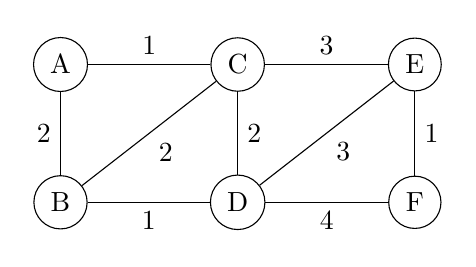
\begin{tikzpicture}[node distance = {1.0cm and 1.5cm}, v/.style = {draw, circle}]
  \graph[nodes={circle, draw}, grow right=2.25cm, branch down=1.75cm]{
    A -- ["1"] C -- ["3"] E,
    B -- ["1",swap] D -- ["4",swap] F,
    B -- ["2"] A,
    C -- ["2"] {D,B},
    D -- ["3",swap] E -- ["1"] F
  };
\end{tikzpicture}
\end{center}

\section{Algoritmos} \noindent 
A continuación se presentan algunos algoritmos para resolver el problema de apareamiento máximo de aristas.

\subsection{Algoritmo voraz}
\subsection{Algoritmo Hopcroft–Karp}

\section{Aplicaciones} \noindent

\section{Resolver caso} \noindent

\newpage
\nocite{*}
\bibliographystyle{ieeetr}
\bibliography{bibliography/ref}
\end{document}
